\section{Design of protocol}
\label{sec:protocol}
\subsection{Overview of proposed scheme}
The procedure of PRIOIDC can be divided into two parts: Initiating registration and Login procedure. Login procedure contains user login, client\_id negotiation, dynamic registration and token obtaining. The overview is shown in Figure~\ref{fig:overview}
\begin{figure}
  \centering
  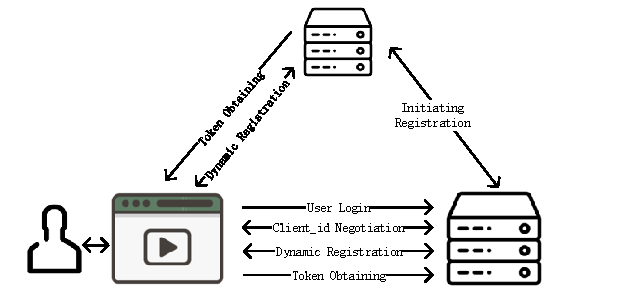
\includegraphics[width=\linewidth]{fig/prioidc.pdf}\label{fig:overview}
  %\subfigure[Authorization Code Flow]{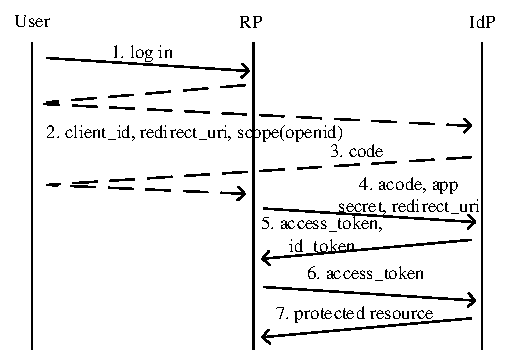
\includegraphics[width=\linewidth]{fig/openidconnect2.pdf}\label{fig:OpenID_code}}
  %\subfigure[Hybrid Flow]{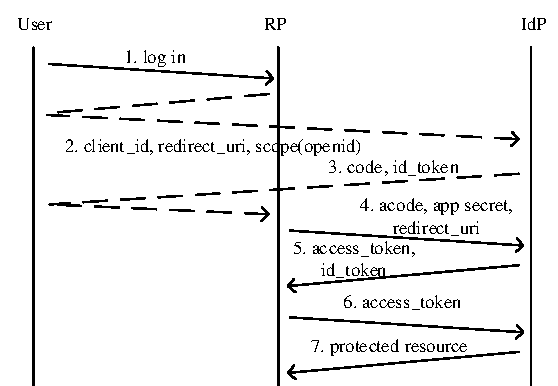
\includegraphics[width=\linewidth]{fig/openidconnect3.pdf}\label{fig:OpenID_hybrid}}
  \caption{Overview of System}
  \label{fig:overview}
\end{figure}
\begin{itemize}
\item[---] Initiating Registration: RPs and users register at IdP. IdP generates unique basic\_client\_id for each RP and unique user id for each user.
\item[---] User Login: User starts log in an RP. If user is labeled as logged in, RP is going to offer service to user. Otherwise RP requires user to start SSO procedure. 
\item[---] Client\_id Negotiation: For each SSO procedure, RP is going to start client\_id negotiation with user. Client\_id is a random number generated by client-id-generating algorithm unrelated with any RP. A client\_id represents login from a user to an RP.
\item[---] Dynamic Registration: To make the client\_id generated by negotiation between user and RP, user is going to register client\_id at IdP by the dynamic registration API provided by IdP. IdP is going to check whether client\_id is unique and ask RP to restart client\_id negotiation for another client\_id.
\item[---] Token Obtaining: After dynamic registration success, RP is going to redirect token request to IdP. IdP firstly authenticates user and then generates id token for RP. Id token contains RP's client\_id and user id. Client\_id is provided by RP and user id is generated through sser-id-generating algorithm by IdP. RP is able to get the constant user identity from user id.
\end{itemize}

\subsection{Client-id-generating and User-id-generating algorithm}
Client-id-generating and User-id-generating algorithm are created based on Discrete Logarithm problem\cite{shiu2007cryptography:}.
%需要解释离散对数吗?
IdP carefully chooses a big prime \emph{p}\cite{rfc3526} for system. When a RP initialize registration at IdP, IdP will provide RP a unique primitive element module \emph{p}. It's used in RP as the basic\_rp\_id and RP will generate another primitive \emph{g} from basic\_rp\_id for further client\_id negotiation. As \emph{p} is a prime and \emph{a} is a primitive element module \emph{p}, if $\alpha$ is a relatively prime of \emph{p-1}, $a^\alpha mod p$ is another prime element module \emph{p}.

For each login process, the user and RP negotiate the temporary $client_{id}$ for the RP registration at the IdP.
While starting a login procedure, there is \textbf{Diffie-Hellman key Exchange}\cite{DiffieH76} between RP and user. Firstly RP sends $pk\_rp=g^x mod p$ to user, and \emph{x} is a random number. After receiving the pk\_rp, user continue generating the random number \emph{y} until $r=pk\_rp^y mod p$ is a relative prime of \emph{p-1}. Then user sends $pk\_user=g^y mod p$ to RP so that both user and RP can get $r=g^{xy} mod p$. So the client\_id is generated as: $$client\_id=basic\_rp\_id^r mod p$$ such that client\_id is another primitive element module \emph{p}.

To identify users, IdP keeps a unique id for each user. After receiving a client\_id, IdP will generate the one-to-one correspondence user\_id$$user\_id=client\_id^{id} mod p$$so$$user\_id=basic\_rp\_id^{r\cdot id}modp$$
As \emph{r} is a relative prime of \emph{p-1}, according to \textbf{Extended Euclidean} algorithm RP can get $r^{-1}$ and let $1=r\cdot r^{-1} mod (p-1)$. While receiving user\_id from IdP, RP can get a user identity $$user\_rp\_id=user\_id^{r^{-1}} mod p$$so$$user\_rp\_id=basic\_rp\_id^{id} mod p$$For one user in a RP, user\_rp\_id is constant. But  user\_rp\_ids are disparate in RPs because basic\_rp\_ids are different in each RP.

\subsection{Login flow}
User firstly logs in an RP. If RP find that user is unauthenticated, RP is going to negotiate a new client\_id with user. Then user starts dynamic registration and forward the registration result from IdP to RP. If registration succeeds RP will construct a token request and redirect user to IdP. IdP authenticates user and generates an id\_token of user for RP. Id\_token is sent to RP and RP gets user\_rp\_id from id\_token. RP is going to identify the user through user\_rp\_id. 

%抵抗phishing攻击:一定需要正确的RP参与,攻击者作为中间人
%1.使用IdP提供应用basic_rp_id与url的绑定,user agent保存映射
%缺点:占用空间,user agent需要缓存整个映射
%2.RP与用户通过加密的通道传输redirect_uri

%如果由RP选择basic_rp_id,那么多个rp之间的basic_rp_id有幂次关系,那么就可以关联用户

\subsubsection{Initiating Registration}
If an RP wants to join the SSO system, it must do the initialization registration at IdP. 
As well as traditional SSO system, IdP is going to inspect the real identity of RP and store RP's information on IdP's server.
During registration procedure RP sends its URL for id\_token acceptance to IdP. IdP generates a unique primitive element module \emph{p} for RP as basic\_rp\_id. Then IdP puts basic\_rp\_id, URL and the prime \emph{p} together and encodes them to Json Web Token. This token is called rp\_certificate. A typical rp\_token carries the following information:
\begin{lstlisting}[language={[ANSI]C},%frame=shadowbox, 
   basicstyle=\ttfamily]  
    {
        "alg": "RSA",
        "type": "certificate"
    }.
    {
        "iss": IdP URL,
        "sub": basic_rp_id,
        "name": RP name,
        "redirect_uri": URL
    }
\end{lstlisting} 

Same as RP, user need to register at IdP. IdP is going to generate unique user id for each user during registration. 
\subsubsection{Client\_id Negotiation}
An attacker is able to be the man in the middle between RP and user in client\_id negotiation using phishing attack. When a user logs in attacker's website, attacker logs in another RP as a user. In client\_id negotiation, attacker just transmits user and RP's requests and responses to each other. As a result, attacker shares the same client\_id with user and RP and gets a id\_token valid in RP from user.
So besides of generating client\_id, RP has to send its rp\_certificate to user in this phase. It protects user from sending id\_token to malicious opponent. As rp\_certificate contains RP's name, it allows user can identify the real RP's identity when doing login.
\subsubsection{Dynamic Registration}
User generates IdP's registration URL by \emph{iss} from rp\_certificate. 
The client\_id negotiation is described in client-id-generating algorithm. Dynamic registration starts after client\_id negotiation. User generates a random redirect\_uri and sends it to IdP as well as client\_id. IdP checks the uniqueness of client\_id and sends the result success or fail back. If registration fails, user is going to restart client\_id negotiation. Otherwise user will forward the registration response to RP.  
\subsubsection{Obtaining Token}
RP firstly redirects user to IdP with its token request. User generates IdP's authenticate URL by \emph{iss} from rp\_certificate and compared it with RP's redirect location. If they point the same address, user is going to continue the login.
To keep the advanced protocol same as OpenID Connect 1.0, after authenticating a user IdP is going to redirect the user to the redirect\_uri of RP with id\_token as parameter. As redirect\_uri is random, user stops the redirection. User then sends id\_token to the URL received from client\_token negotiation to defend man-in-the-middle attack. RP gets user\_id from id\_token and gets user\_rp\_id computed from user\_id. If it's the first time user logs in RP, RP is going to finish the registration. Otherwise RP searches user profile through user\_rp\_id. 
%\subsection{Roles' Ability Demands}
%\emph{Demands on IdP}. 